\documentclass{article}
\usepackage{graphicx}
\usepackage{float}
\usepackage{amsmath}
\usepackage{amsfonts}
\usepackage{amssymb}
\usepackage{hyperref}
\usepackage{esint}
\usepackage[utf8]{inputenc}
\usepackage[a4paper, portrait, margin=0.75in]{geometry}
\setlength\parindent{0pt}
\usepackage[italian]{babel}



\hypersetup{
    colorlinks=true,
    linkcolor=black,
    filecolor=magenta,
    urlcolor=blue,
    pdftitle={Tecnologie internet},
    pdfpagemode=FullScreen,
}


\begin{document}
    \author{kanopo}
    \title{Ingegneria dei software}

    \maketitle
    \tableofcontents

    \listoffigures
    \listoftables

    \newpage

\section{T1 - Software Development Process}
L'Ingegneria del Software non è solo scrivere codice è piuttosto un concetto 
di risoluzione dei problemi del mondo reale sfruttando il software.

I requisiti sono sempre più stringenti: tempi brevi, sistemi complessi, molte features.

Un buon software deve avere ottime \textbf{maintenability, dependability, efficiency, acceptability}.

I problemi e le soluzioni sono sempre complesse ma il software permette massima flessibilità.
È un sistema discreto.

Le sfide principali sono rappresentate da \textbf{eterogeneità, delivery, trust}.

La fase di problem solving si suddivide in analisi e sitesi.

\subsection{Cos'è l'ingegneria del software?}
L'Ingegneria del software è un \textbf{insieme di tecniche, metodologie, strumenti} che aiutano
nella produzione di software di alta qualità dati un budget, una scadenza, e delle modifiche continue.

La sfida principale è quelli di aver a che fare con complessità elevate e ad un aumento delle
responsabilità, dato che un ingegnere del software non deve solo scrivere codice, ma piuttosto lavorare
con competenza e confidenzialità, attenendosi ad un'etica.

\subsubsection{Processo del software}
Dopo una rappresentazione astratta, si procede con un set di attività strutturate:
specifiche dei \textbf{requirements, design, implementazione, validazione, evoluzione.}

\subsection{Modelli di sviluppo del software}
Distinguiamo tra \textbf{plan-driven} e \textbf{agile} development. Nel primo si pianificano 
i requisiti e solo in seguito si sviluppa il software. Nel secondo si sviluppa il software un pezzo alla
volta, a stretto contatto con il cliente per dei feedback.

\subsubsection{Modello a cascata}
Modello plan-driven, le specifiche e lo sviluppo sono separati.

I pro:
\begin{itemize}
    \item ottima documentazione
    \item manutenzione semplice
\end{itemize}

I cons:
\begin{itemize}
    \item specifiche congelate dopo la pianificazione iniziale
    \item cliente poco coninvolto
    \item tempi lunghi
\end{itemize}

\begin{figure}[h!]
    \centering
    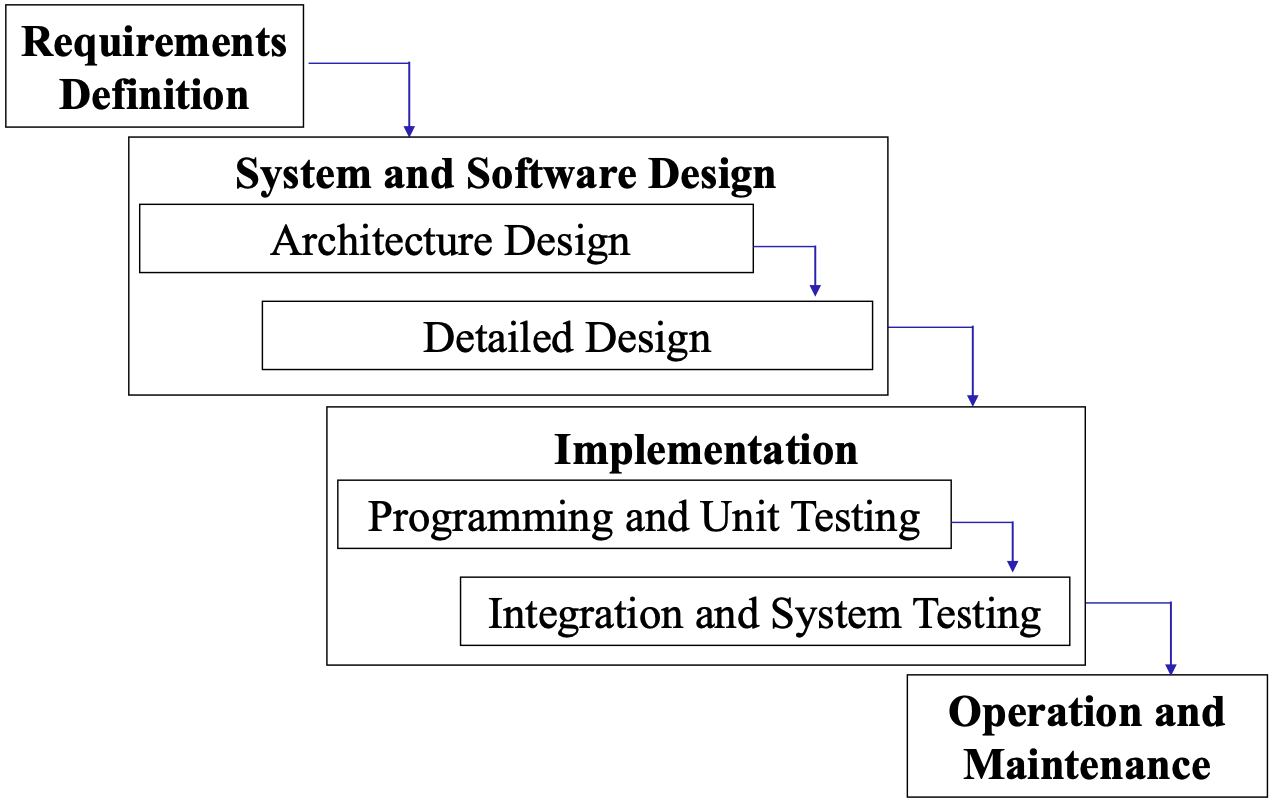
\includegraphics[width=0.5\linewidth]{imgs/1 - cascata.png}
    \label{fig:modello_cascata}
    \caption{Modello a cascata}
\end{figure}

\subsubsection{Modello a spirale}
Diverse fasi che susseguono a spirale, la gestione del rischio viene gestita
tramite prototipazione che permette di testare i prodotti.

I pro:
\begin{itemize}
    \item prevenzione dei rischi
    \item completezza della documentazione
    \item flessibilità
    \item elevata usabilità
    \item buon design
    \item facilità di manutenzione
    \item ridotto costo di sviluppo
\end{itemize}

I cons:
\begin{itemize}
    \item modello costoso
    \item riservato ad esperti e a progetti costosi
\end{itemize}

Il prototipo è un'implementazione limitata del sistema, rappresentanti solo alcuni aspetti alla volta.

\begin{figure}[h!]
    \centering
    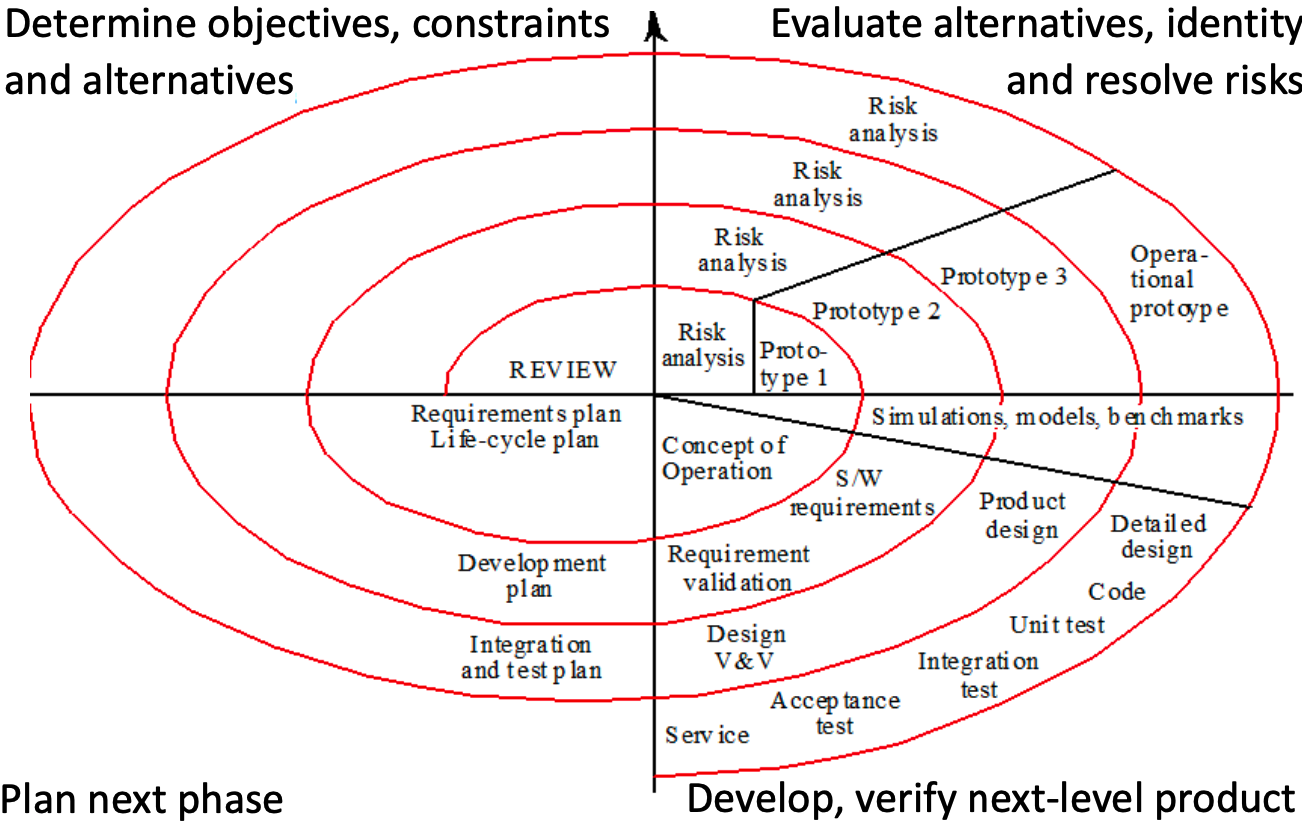
\includegraphics[width=0.5\linewidth]{imgs/2 - spirale.png}
    \label{fig:modello_spirale}
    \caption{Modello a spirale}
\end{figure}

\subsubsection{Sviluppo incrementale}
Modello che si suddivide in fasi:
\begin{enumerate}
    \item raccolta dei requisiti
    \item versione iniziale
    \item fase di design
    \item fase di implementazione
    \item produzione di versione finale
\end{enumerate}

I pro:
\begin{itemize}
    \item naturale presenza di prototipi ad ogni aggiunta di features
    \item basso rischio di fallimento
    \item qualità di testing in base alla priorità
\end{itemize}

I cons:
\begin{itemize}
    \item scarsa visibilità d'insieme
    \item sistemi mal strutturati
    \item skill speciali necessarie
\end{itemize}

Adatto a progetti piccoli o parti di progetti grandi.

\begin{figure}[h!]
    \centering
    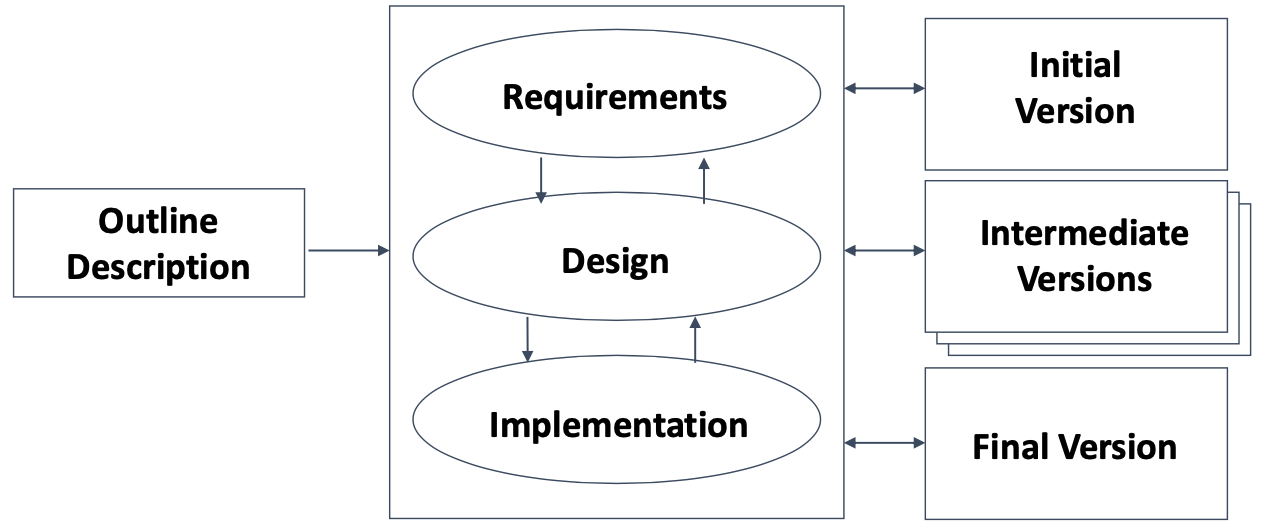
\includegraphics[width=0.5\linewidth]{imgs/3 - incrementale.png}
    \label{fig:modello_incrementale}
    \caption{Modello a incrementale}
\end{figure}

\subsubsection{Sviluppo guidato dai test}
Vengono prima scritti i test e poi l'implementazione mettendo le difficolta in primo piano.

Rende il debug più semplice.

Si aggiunte il nuovo test e poi la features cosi da veriicare che tutti i test 
precedenti siano validi.

\subsubsection{Sviluppo agile}
Questo modello di sviluppo è basato sul concetto di delivery del prodotto continuo 
avendo delle features in continua evoluzione.

Il cliente è al centro dello sviluppo, il team si autoorganizza e le features 
vengono aggiunte man mano.

Essendoci la mancanza di planning il team deve essere esperto per non perdersi.


Spesso si creano documentazioni sbagliate o incomplete.

\subsubsection{Extrem programming}
L' XP viene scelte quado i requisiti cambiano velocemente, i team sono ridotti
e affiatati(pair programming per esempio).

Tipo di programmazione agile, basato sul design semplice, release minori,
refactoring continuo, alta semplicità.

\begin{figure}[h!]
    \centering
    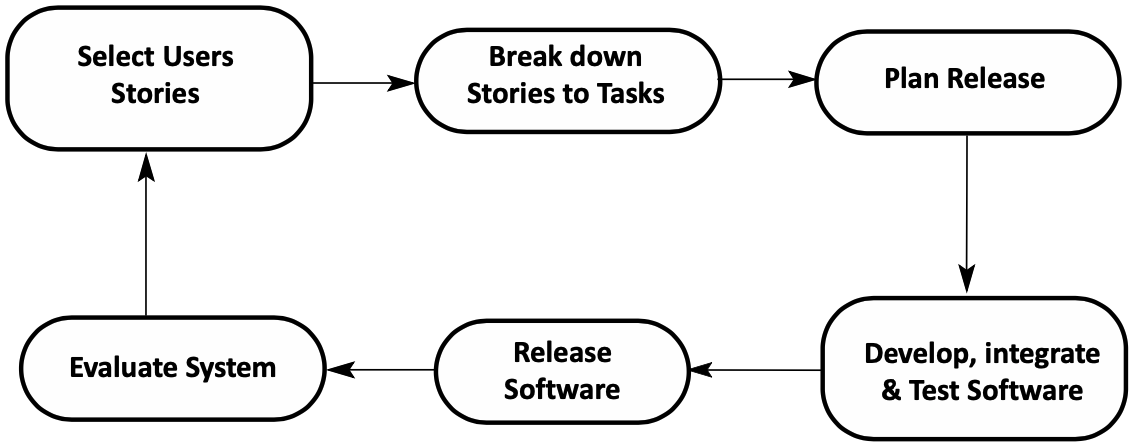
\includegraphics[width=0.5\linewidth]{imgs/4 - xp.png}
    \label{fig:modello_xp}
    \caption{Modello a extrem programming}
\end{figure}

\subsection{Software riusabile}

È comodo lavorare per \textbf{microservizi atomici}, di modo da usarli in seguito 
se si affronta un problema simile, un'esempio sono le API, è sempre meglio riusare qualcosa 
che riscriverlo da zero.

Questo "\textit{mindset}" riduce i temi e i costi di sviluppo nel luno periodo.

Il contro è il fatto che i microservizi non sono fatti espressamente per una task specifica
e si va a sacrificare qualche requisito.


\section{T2 - Coding, Debugging, Testing}
Lo stile di coding è importante perchè un programma viene scritto una volta e letto
spesso da altri!

Stare a ttenti ai layout, nomi, commenti, ecc\dots

\subsection{Legge di Ambler per gli standard}
Più uno standard è adottato e più sarà facile farlo usare al proprio team.

Non perdere tempo adietro a standard scemi.

Se hai dei dubbi usa gli standaard di google che sicuramente ne sanno più di me e te.
\textbf{\href{https://google.github.io/styleguide/}{standard di google}}


Solitamente si hanno degli standard aziendali e questi standard vanno a chiarire aspetti come:
\begin{itemize}
    \item nomenclatura
    \item formattazione
    \item formato
    \item contenuto
\end{itemize}

\subsection{Coding practices}
\begin{itemize}
    \item indentazione
    \item whitespaces
    \item naming, commenting
\end{itemize}

Fondaentale è spiegare i compiti delle classi, funzioni e procecssi complessi.

Utilizzare uno standard permette ai collechi di non dover riscrivere il codice.
Rendendo più semplice le iterazioni del codice successive.

\subsection{Gestione degli errori}
Si fa un distinguo fra il prima, durante e dopo:
\begin{itemize}
    \item prrevenzione
    \item rilevamento
    \item recupero
\end{itemize}

Per debuggare, bisogna riconoscere l'errore, isolare la fonte, identificarne la causa,
trovare un fix, applicarlo e testarlo.

\subsection{Testing}
Permette di trovare errori ma non la loro assenza, \textbf{il tester non dovrebbe
essere il programmatore}.

\subsubsection{Unit testing}
Test di singoli componenti.

\subsubsection{Integration testing}

L'intero sistema è visto come insieme di sottositemi, l'obbiettivo è quello di testare tutte le interfacce e le 
interazioni fra i sottositemi.

\subsubsection{System testing}
test dell'intero sistema per vedere se rispetta i requisiti funzionali.

\subsubsection{Functional testing}

Verifica delle funzionalità del sistema, test basati sui requisiti del progetto.

\subsubsection{Performance testing}
Test in situazioni estreme(stress testing, volume testing, recovery testing, penetration testing).

\subsubsection{Acceptance testing}
Il sistema è pronto per la produzione??

Test scelti ed effettuati dal cliente.(alpha e beta test)

\section{T3 - System Modelling and UML}

Rappresentazione astratta del sistema e dei problemi, si dedvono introdurre i componenti essenziali mediante una noazione
consistente.

Il system modelling deve essere \textbf{predictive}(prima del development), \textbf{extracted}(da un sistema 
esistente) e \textbf{prescriptive}(definire regole per l'evoluzione del software).

\subsection{UML}
UML è semplice, espressivo, utile, consistent, estensibile.

\section{T4 - Requirements engineering}

Gli scopi dell'ingegnerizzazione dei requisiti è \textbf{identificare} i servizi necessari
e i constrait, \textbf{definire} offerta e contratto, \textbf{ottenere} tutte le informazioni
necessarie al design.

Si cerca di ottenere requirements:
\begin{itemize}
    \item validi(reali necessità)
    \item non ambigui
    \item completi
    \item comprensibili
    \item consistenti
    \item prioritizzati
    \item verificabili
    \item modificabili
    \item tracciabili
\end{itemize}

\subsection{Classificazione dei requirements}
\subsubsection{Requisiti funzionali(features di sistema)}
Descrivono funzionalità di sistema o di servizio, come input di dati, output, 
operazioni svolte, workflow, autorizzazioni.

\subsubsection{Requisiti non funzionali(features di sistema)}

Descrivono i limitti di parti del sistema e del suo sviluppo.

Specificano criteri per giudicare l'operato del sistema.

\subsubsection{Requisiti del dominio(features di sistema)}
Derivato dal campo di utilizzo del software.

\subsubsection{Requisiti volatili(natura statica/dinamica)}
\begin{itemize}
    \item mutable requirements = cambiano nel tempo(tasse, nomative, ecc)
    \item emergent requirements = cambiano quando il cliente capisce di più il sistema
    \item consequential requirements = emergono con l'informatizzazione del sistema che non lo era
    \item compatibility requirements = emergono dal dover interfacciare il sistema con altri sistemi 
\end{itemize}

\subsection{Rischi}
I rischi della stesura dei requisiti possono essere:
\begin{itemize}
    \item imprecisioni
    \item conflitti tra requisiti
\end{itemize}

\subsection{Documento di specifica dei requirements}

Questo documento specifica i requisiti del sistema, includendo una definizione
e una specifica.

Prende il nome di system specification se include direttive su harware e software.

Software Requirements Specification (\textbf{SRS}) se include solo specifiche software.


Un \textbf{SRS} deve includere:
\begin{itemize}
    \item introduzione
    \item descrizione generale
    \item features
    \item requirements
\end{itemize}

Il linguaggio naturale usato per stilare questo documento implica ambiguità,
per questo si ricorre a una struttura ben definita per evitare ambiguità.

\section{T5 - Requirements ecgineering and UML}
\subsection{Use case diagram}
In questo diagramm vengono inclusi tutti i casi di utilizzo del sistema,
da parte dei vari attori che rappresentano gli utenti.

Il \textbf{System boundary} divide l'interno dall'esterno del sistema.

\subsection{Class diagram}

Diagramma che rappresenta le classi tramite:
\begin{itemize}
    \item gli attributi(pubblici con +, privati con - e \# per i protetti)
    \item le funzioni delle classi
\end{itemize}

\subsubsection{Associazione}
Quando una classe svolge il ruole di variabile all'interno di un'altra classe,
questa connessione deve essere rappresentata, si usano:
\begin{itemize}
    \item cardinalità
    \item direzione
    \item constraint
    \item ruoli
\end{itemize}

\begin{figure}[h!]
    \centering
    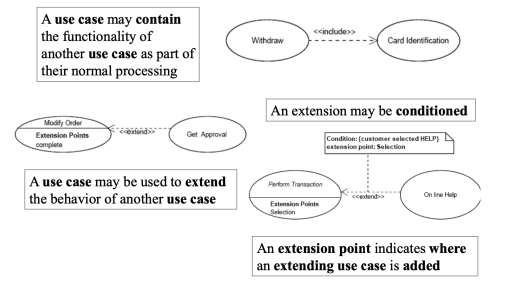
\includegraphics[width=0.5\linewidth]{imgs/5 - associazione.png}
    \label{fig:associazione}
    \caption{Associazioni}
\end{figure}

\pagebreak
\subsubsection{Gneralizzazione e nesting}

La generalizzazione indica \textbf{eretidarietà}, nesting indica che una classe 
è nestata nella classe dove arriva l'operatore.

\begin{figure}[h!]
    \centering
    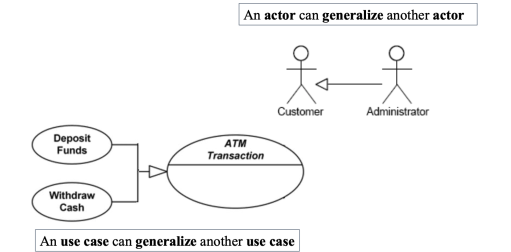
\includegraphics[width=0.5\linewidth]{imgs/6 - generalizzazione e nesting.png}
    \label{fig:generalizzazione_nest}
    \caption{generalizzazione e nesting}
\end{figure}

\subsubsection{Dipendenza e realizzazione}
\begin{itemize}
    \item \textbf{dipendenza} = relazione debole tra client e supplier
    \item \textbf{realizzazione} = relazione tra specifica e implementazione
\end{itemize}

\subsubsection{Aggregazione e composizione}

L'aggregazione rappresenta un elemento composto da altri elementi minori.


\begin{figure}[h!]
    \centering
    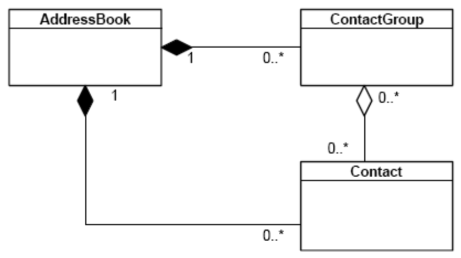
\includegraphics[width=0.3\linewidth]{imgs/7 - aggregazione.png}
    \label{fig:aggregazione}
    \caption{Aggregazione e composizione}
\end{figure}

\subsection{Sequence diagram}
Usa un timeline verticale per rappresentare l'interazione tra le classi.

Ci possono essere comunicazioni sincrone e asincorne.
\subsection{Activity diagram}
Diagramma che rappresenta un'operazione eseguita nel sistemasa con rappresentazione
dell risorse utilizzate(io, disk, banda, ecc)

\subsection{Robustnes diagram}

Diagramma UML semplificato che appresena gli use cases verificandone la corretteza, 
completezza e requisiti.

\section{T6 - Feasability and requirements elicitation}
Per ottenere le informazioni necessarie dobbiamo identificare le fonti, acquisire i dati,
verificarli e sintetizzarli.

Le varie persone interessate al progetto possono essere suddivise cosi:
\begin{itemize}
    \item stakeholder: interessato nel progetto
    \item developer: produce con pochi errori
    \item project managment: budget, scadenze
    \item investor: velocizzazione del progetto
    \item cliente e utente: usabilità e workflow
\end{itemize}


\subsection{Tecniche di elicitation}
(elicitation = tirare fuori le informazioni)
\subsubsection{Document analysis}

Analizzare i documenti e insieme agli stakeholder verificare la correttezza dei dati.

\subsubsection{Observation of the work environment}
Apprendere informazioni importanti osservando il lavoratore.
\subsubsection{Questionario}
Determinare i fatti e leopinioni con un questionario.
\subsubsection{Interviste}
Decidere chi intervistare e acquisire i dati.
\subsubsection{Scenari e casi di utilizzo}
Esempi IRL(In Real Life) di come il sistema verrà usato.

\subsection{Attività di supporto all'elicitation}
\subsubsection{Brainstorming}
composto dalle fasi storm(spara idee) e calm(analizza idee)
\subsubsection{Focus group}
simile al brainstorming
\subsubsection{Prototipi}
Esecuzone di una task e si analizza lasituazione facendo emergere problemi
e soluzioni.

\section{T7 - Use cases}

Gli use cases sono scenari plausibili che sfruttano i diagrammi UML.

Ogni requirements deve essere mappato da almeno un use case.


\subsection{Componenti principali}
Lo use case deve definire lo stato precedente del sistema,
l'ordine degli eventi, le alternative, situazioni eccezionali e i risulati.
Deve menzionare gli attori che prendono parte al sistema, i problemi di design,
i diagrammi di relazione. 

Ecco delel guidelines:
\begin{itemize}
    \item non pensare all'implementazione
    \item essere pessimistici
    \item elencae gli scenari funzionanti
    \item elencare tutti i possibili use cases
    \item utilizzare un formaato standard
    \item utilizzare verbi appropriati
    \item documentare bene le situazioni eccezionali
    \item non rappresentare singoli step come use cases
\end{itemize}



\begin{figure}[h!]
    \centering
    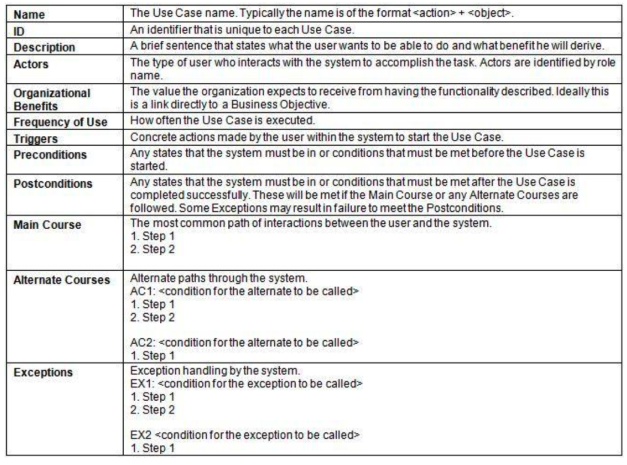
\includegraphics[width=0.6\linewidth]{imgs/8 - use case template.png}
    \label{fig:use_case}
    \caption{Tamplate per i casi di utilizzo}
\end{figure}

\section{T8 - Requirements}
L'analisi dei requisiti permette di raffinare e strutturare i requisiti in 
modo da renderli più chiari, precisi e formali.


\subsection{Analysis classes}
Il concetto è quello di astrarre le entità del problema.

\subsection{Classes discovering techniques}
\subsubsection{Noun verb analysis}
Analisi che sfrutta i contenuti delle specifiche del progetto.
Necessita di completezza del documento molto alta.

\subsubsection{Use case driven approch}
Approccio che sfrutta fli scenari degli use cases.
\subsubsection{Common class patterns}
Analisi basata sulla teoria della classificazione generica degli oggetti.

Fornisce linee guida, ma non un processo sistematico per ottenere le classi.


Introduce errori di mal'interpretazioni.

\subsubsection{CRC cards}
Sono usate in specifiche sessioni di brainstorming, generalmente si 
parte dagli use cases e s icreano delle card con:
\begin{itemize}
    \item class name
    \item responsabilities
    \item collaborators
\end{itemize}

Non è un metodo sistematico, si usano le CRC cards come validazione.

Gli achievement di questo metodo sono:
\begin{itemize}
    \item Verifica la corretteza dello use case
    \item verifica la correttezza delle associazioni
    \item verifica la corretteza delle generalizzazioni
    \item trovare le classi omesse
    \item scovare opportunità di refactoring
\end{itemize}

\subsubsection{Mixed approch}
Migliore:
\begin{enumerate}
    \item Le classi iniziali provengono dalla conoscenza del dominio
    \item si sfrutta come guida il common class pattern
    \item per aggiungere altre classi si usa la noun verb analysis
    \item per verificare il lavoro si usano gli use cases
    \item per il brainstorming si usano le CRC cards
\end{enumerate}


\section{T9 - Requirement validation and managment}
\subsection{Valdation}
La validazione consiste nella verifica della correttezza dei requisiti, con obbiettivi
la completezza e i costi.
\begin{itemize}
    \item consistenza
    \item realismo
    \item verificabilità
\end{itemize}
\subsection{Requirements managment}
Si verificano gli errori, conflitti e inconsitenze.

Soddisfare il cliente e mantenere i costi bassi:
\begin{itemize}
    \item identificazione dei requisiti
    \item processo di modifica
    \item policy di tracciabilità
    \item supporto del case tool
\end{itemize}
\subsubsection{Case tool support}
non ho voglia di spiegarlo.
\subsubsection{Stati dei requirement}
tutto questo ambaradam è molto simil ad un issue tracker come git.
\begin{itemize}
    \item proposal
    \item approved
    \item rejected
    \item implementation
    \item verified
    \item deleted
\end{itemize}

Si fanno sostanzialemnte dei test con un version control e si fa il roll back
in caso di problemi.

\subsubsection{Tracciabilità}
Anche questo discorso viene gestito bene da un software tipo git.

\subsubsection{Traciability planning}
Elemeti fondamentali del planning:
\begin{itemize}
    \item tipi di stakeholder
    \item informazioni richieste
    \item dove e da chi raccogniere info
    \item dove e come mantenere le info
    \item dove e come cercare le info
\end{itemize}

Ci sono delle limitazioni per il plannign:
\begin{itemize}
    \item numero di requirements
    \item lifetime stimato
    \item livello di maturità dell'azienda
    \item dimensione progetto
    \item altri vincoli dell'utente
\end{itemize}
\setcounter{section}{11}
\section{T12 - Object constraint lenguage}
Fa parte delle specifiche UML, e segue uno standard di IBM, è un linguaggio 
formale usato per descrivere i modelli Object oriented.
\subsection{Model type}
sono classi, subclasses, classi di associazione, interfacce ed enumerazioni.

Hanno proprietà e attributi.
\subsection{Operazioni, espressioni, constraint}
I constraint sono dei valori booleani che veificano una condizioni, servono
a porre limitazioni sul tipo di valore che può avere una classe.

\begin{itemize}
    \item Migliorano la documentazione
    \item più precisione
    \item comunicazione senza ambiguità
\end{itemize}

Vari tipi di constraint:
\begin{itemize}
    \item invarianti(quando l'istanza è a riposo)
    \item precondizionali
    \item postcondizionali
    \item guard(vera prima e dopo)
\end{itemize}

\section{T13 - Design process}
Processo che permette di capire come implementare il sistema.

Si parte dai requirements e si tiene conto dei design general princilas.

\subsection{Linee guida}
\begin{itemize}
    \item esibire organizzazione modulare che fa uso intelligente di controllo tra componenti
    \item partizione in componenti logici
    \item descrivere sia dati che procedure
    \item arrivare ad interfacce che riducono la complessità
\end{itemize}

Un buon design deve implementare tutti i requirement espliciti del modello di analisi, e tutti quelli impliciti
desiderati dal cliente. Dev'essere leggibile e comprensibile, sia per chi scrive codice, sia per chi lo testa
e supporta. In generale, dovrebbe dare un'immagine generale del software, indicandone i dati, i domini
funzionali e behavioral dal punto di vista dell'implementazione.



\subsection{Stadi del design process}
\begin{enumerate}
    \item comprendere il problema
    \item identificare una o più soluzioni
    \item processo iterativo ed incrementale
\end{enumerate}

\subsection{Design as series of decisions}
Alcuni tradeoff possono essere:
\begin{itemize}
    \item funzionalità vs usabilità
    \item costo vs robustezza
    \item efficienza vs portabilità
    \item velocità di sviluppo vs funzionalità
    \item costo vs riutilizzabilità
\end{itemize}

Gli step per una decisione pesata sulle priorità sono:
\begin{enumerate}
    \item Elencare le alternative possibili
    \item elencare i pro e i contro di ogni alternativa(rispetto agli obiettivi e alle priorità)
    \item determinare se alcune alternative impediscono altri obiettivi
    \item scegliere l'alternativa che permette di raggiungere più obiettivi
    \item aggiustare la priorità per decisioni future
\end{enumerate}

\subsubsection{Approcci}
Approccio \textbf{top-down}: prima si fa il design ad alto livello del sistema,
poi si prendono le decisioni man mano che si sviluppa il sistema.


Approccio \textbf{botton-up}: prima si decidono le utilities di basso livello riutilizzabili,
poi il modo di integrarle insieme.


Approccio \textbf{mixed}: si usa top-down per scegliere la struttura ed 
il bottom-up per i componenti riutilizzabili.

\subsubsection{Attività, rischi e obiettivi}

La fase di design ha tre fasi:
\begin{itemize}
    \item design dell'architettura
    \item user interface
    \item class design
\end{itemize}

Un buon design è \textbf{flessibile, dettagliato, ben documentato e buona possibilità di managment}.

\section{T14 - Design concepts}

Un sistema sftware ha diversi possibili problemi:
\begin{itemize}
    \item rigidità
    \item fragilità
    \item immobilità(difficle riusare i componenti)
    \item viscosità(più semplice l'hack del mantenimento del design originale)
\end{itemize}


\subsection{Software design concepts}
\subsubsection{Abstraction}
L'astrazione permette di focalizzarsi su parti importanti del software senza perdersi nell'implementazione.

Permette la descrizione di un sistema come struttura a
livelli.

\subsubsection{Refinement}
processo top-down iterabile che ad ogni passo trasforma istruzioni generiche in istruzioni più specifiche.
\subsubsection{Nascondere le informazioni}


L'information hiding è strettamente legato a:
\begin{itemize}
    \item astrazione
    \item coupling
    \item coesione
\end{itemize}

\subsubsection{Modularità}

Un metodo di design può essere detto modulare solo se supporta:
\begin{itemize}
    \item decomposability(ridurre in modulli più piccoli)
    \item composability(accorpare in un unico modulo)
    \item understandability(un modulo è comprensibile senza sapere gli altri)
    \item continuity(la modifica in un modulo modifica solo lui)
    \item protection(bug in un modulo?? affligge solo qul modulo!)
\end{itemize}

I principi per il design modulare sono: linguistic modular units (i moduli devono corrispondere alle
unità del linguaggio, come pacchetti o moduli), poche interfacce, poco scambio di informazioni tra
moduli, interfacce esplicite (se due moduli comunicano, dev'essere ovvio), information hiding(tutte
le informazioni di un modulo dovrebbero essere private, se non specificatamente dichiarato il contrario, e
per l'accesso bisogna utilizzare interfacce).


\subsubsection{Coesione}
La coesione misura la chiusura di una relazione tra elementi di un componente/classe. Una coesione forte
è desiderabile perché semplifica le correzioni, le modifiche, le estensioni, riduce il testing e promuove il
riutilizzo. Abbiamo più livelli di coesione (dal più basso al più alto):
\begin{itemize}
    \item coincidental(elementi senza relazioni ma uniti per convenienza)
    \item logical(elementi che fanno cose simili)
    \item temporal(elementi attivi nello stesso tempo)
    \item procedural(elementi che compongono una singola sequnza di controllo)
    \item communicational(elementi con stesso input e stesso output)
    \item sequential(l'output di uno è l'input dell'altro)
    \item functional(elementi che soppriscono ad un funtiona lrequirement)
    \item object(operazioni tra oggetti)
\end{itemize}

\subsubsection{Coupling}

Misura l'interconnessione tra moduli. Quando è debole, i moduli sono fortemente indipendenti. Livelli di
coupling dal più debole al più forte:
\begin{itemize}
    \item no direct(nessuna dipendenza)
    \item data(solo dati necessari)
    \item stamp(passati una lista di argomenti ma solo alcuni vengono usati)
    \item control(si passano flags e altri paramentri)
    \item externl(legato a device o device drivers)
    \item common(uso di dati globali)
    \item content(modificadi dati dell'altro modulo)
\end{itemize}

Con coupling elevato i componenti sono difficili da comprendere autonomamente,
le modifiche causano bug in altri moduli e il riuso di moduli fa schifo.

Con coupling basso aumentano i costi di performance ma lo sviluppo ne gode.


\section{T15 - Objects oriente design principles}
\subsection{Principi dell'Object Oriented Design}
\subsubsection{SRP - Single Responsability Principle}
Una classe deve avere una sola ragione di cambiare.

Le modifiche ai requirements si mappano sulle responsabilità.

Avere tante classi con responsabilità separate semplifica e rende il design flessibile.

\begin{quotation}
    \textit{
        In programming, the Single Responsibility Principle states that every module or class should have
responsibility over a single part of the functionality provided by the software.
    }
\end{quotation}


\subsubsection{OCP - Open Closed Principle}
Un modulo deve essere aperto verso l'esterno ma chiuso all modifica.

Meglio implementare cose in classi derivate piuttosto che modificae una classe.

\begin{quotation}
    \textit{
        In programming, the open/closed principle states that software entities (classes, modules, functions, etc.)
should be open for extensions, but closed for modification. If you have a general understanding of OOP,
you probably already know about polymorphism. We can make sure that our code is compliant with the
open/closed principle by utilizing inheritance and/or implementing interfaces that enable classes to
polymorphically substitute for each other.
    }
\end{quotation}


\subsubsection{Liskov Substituotion Principle}
Le classi derivate devono adempiere alle funzioni ereditate dalle classi padre
altrimenti se si usa una classe derivata al posto delal padre si generano errori.

\begin{quotation}
    \textit{
        More generally it states that objects in a program should be replaceable with instances of their subtypes
without altering the correctness of that program.
    }
\end{quotation}
\subsubsection{ISP - Interface Segregation Principles}
Avere tante interfacce client-specific è meglio di una generica.

\begin{quotation}
    \textit{
        In programming, the interface segregation principle states that no client should be forced to depend on
methods it does not use. Put more simply: Do not add additional functionality to an existing interface by
adding new methods. Instead, create a new interface and let your class implement multiple interfaces if
needed.
    }
\end{quotation}

\subsubsection{DIP - Dependency Inversion Principles}
I moduli di alto livello non dovrebbero dipendere da quelli di basso livello
ma dovrebbero dipendere da astrazioni.

\subsection{Principi di package cohesion}
\subsubsection{REP - Release/reuse Equivalency Principle}
Per riusare un componente non si fa copia incolla(perchè si perdono le modifiche alla libbreria) ma 
si inserisce il codice mediante una release della libreria e poi si modifica un'istanza.

\subsubsection{CCP - Common Closure Princple}
Le classi che cambiano insieme devono rimanere insieme.

\subsubsection{CRP - Common Reuse Principle}
Le classi che non sono reutilizzabili insieme non dovrebbero essere pacchettizate insieme.

\subsection{Package Coupling Principle}
\subsubsection{ADP - Acyclic Dependencies Principle}
No cicli nel grafico delle dipendenze.

\subsubsection{SDP - Stabel Dependencies Principle}
Ogni volta che un pacchetto cambia, tutti quelli che dipendono da lui devono 
essere validati.

\begin{quotation}
    \textit{
        Ovviamente tu preferisci i pacchetti stabili
    }
\end{quotation}

\subsubsection{SAP - Stable Abstraction Principle}
Il pacchetto perfetto è tanto stabile quanto astratto.

I pacchetti astratti dovrebbero essere responsabili e indipendenti, mentre 
quelli concreti dovrebbero essere irresponsabili e dipendenti.

\subsection{Attività per un buon design}
\begin{itemize}
    \item Dividi e conquista(scompore tutto in processi semplici da fare uno alla volta)
    \item Aumenta la coesione(Un sistema con alta coesione tiene insieme quello che deve stare insieme e lascio fuori il resto)
    \item Ridurre il coupling(meno interdipendenze tra moduli)
    \item Aumenta l'astrazione(meglio nascondere i dettagli e ridurre la complessità)
    \item Aumentare la riusabilità
    \item Riutilizzare design e codice esistente
    \item Programmare con l'idea di flessibilità(modifiche future)
    \item Anticipare l'obsolescenza(pensare alle tecnologie e pianificare la gestione del sistema)
    \item pensare alla portabilità
    \item pensare alla testabilità
    \item sviluppare con l'idea di difendere il software dal'utente.
\end{itemize}

\section{T16 - Design Patterns}

Un design pattern è una soluzione ricorrente ad un problema comune, che può essere usata
in modi diversi. È dipendente da linguaggio ed implementazione. I design patterns hanno vari obiettivi:
\begin{itemize}
    \item Codificare un buon design
    \item dare nomi espliciti alle strutture
    \item ciao
\end{itemize}


















































































































































































\end{document}

